\subsection{Semi-synthetic experiment with NHANES patients}\label{appB3}
\noindent{\bf Data and simulator.}
We build a semi-synthetic benchmark in which the patients are real and only their responses to insulin are simulated. We take the 229 insulin-naive adults with diagnosed diabetes and HbA1c $\ge7\%$ in the National Health and Nutrition Examination Survey (NHANES) 2017--2018 \citep{nhanes2017}, i.e., the patients for whom basal insulin initiation is typically considered (Table~\ref{tab:nhanes_cohort}). Each simulated patient is drawn with replacement from this cohort and keeps their measured baseline HbA1c $A_0$ and body weight $W$.
For a daily basal insulin dose $d_k\in\{0, 10, 20, 30, 40\}$ U/day ($K=4$), the HbA1c after treatment follows an $E_{\max}$ model on the excess HbA1c above $5\%$,
\[Y_k=5+(A_0-5)\Big(1-E_{\max}\frac{S\,d_k}{ED_{50}+S\,d_k}\Big)+\varepsilon,\qquad S=\frac{\bar W}{W}\,e^{\eta},\]
with $E_{\max}=0.7$, $ED_{50}=10$ U/day, $\bar W=86.2$\,kg the median cohort weight, so that the effect depends on the dose per kilogram, $\eta\sim N(0,0.3^2)$ unexplained between-patient variation, and $\varepsilon\sim N(0,0.15^2)$ assay noise shared across doses. With these values, the mean HbA1c reduction is 1.2, 1.5, 1.7, 1.9 percentage points at 10, 20, 30, 40 U/day, respectively (0.12--0.46 U/kg for a patient of median weight), of the same order as the reductions reported when basal insulin is added to oral therapy \citep{riddle2003}. The parameters of the dose response are chosen to be clinically plausible but are not fitted to trial data. We use the ADA target HbA1c $\le7\%$ \citep{ada2025glycemic} as the benefit ($y^u=7.0$) and the intensive target HbA1c $\le6\%$, which increased mortality and severe hypoglycemia in the ACCORD trial \citep{accord2008}, as the harm ($y^l=6.0$).
Since $Y_k$ is decreasing in $k$ for every patient, Assumptions~\ref{MON} and~\ref{MON2} hold. Assumption~\ref{MIN} is not guaranteed because the latent variable $(A_0,W,\eta,\varepsilon)$ is multi-dimensional; because the simulator returns all potential outcomes, we compute the true $\theta^{\text{MNH}}$ from the joint counterfactual outcomes and compare it with the identified expression in Theorem~\ref{theo5}, finding a maximum discrepancy of $1.3\times10^{-3}$.

Table~\ref{tab:nhanes_truth} shows the ground truth. The Benefit criterion is maximized at 40 U/day and the Harmless criterion at 20 U/day, whereas the MND-B is 10 U/day and the MND-H is 10 U/day: 10 U/day is exactly necessary for the largest share (51.1\%) of patients. At 40 U/day, 21.5\% of patients are driven to HbA1c $\le6\%$ and 77.9\% are over-treated, compared with 1.0\% and 5.5\% at 10 U/day.

\noindent{\bf Results.}
We set $T^{\text{initial}}=10$ and $T=10000$, and repeat each experiment 100 times. Table~\ref{tab:nhanes_choice} shows the chosen doses, Figures~\ref{fig:nhanesB} and~\ref{fig:nhanesH} the cumulative regret, and Table~\ref{tab:nhanes_clinical} the outcomes of the trial patients.
MND-B UCB identifies the MND-B in 39\%, 73\% and 100\% of runs with $\kappa=1$, $0.1$ and $0.01$, respectively. Benefit UCB converges to 40 U/day and Harmless UCB to 20 U/day, and the doses chosen by the MED-based methods depend on $\phi$. Compared with Benefit UCB, MND-B UCB ($\kappa=0.01$) administers 9.8 instead of 36.0 U/day on average and reduces over-intensive control (HbA1c $\le6\%$) from 18.7\% to 1.4\% and over-treatment from 73.6\% to 7.2\%, while 53.1\% instead of 80.1\% of patients reach the target. This reflects the trade-off that the MND makes explicit: it targets the dose that is necessary for the largest share of patients rather than the dose that brings the most patients to target.

MND-H UCB identifies the MND-H in 0\%, 0\% and 0\% of runs with $\kappa=1$, $0.1$ and $0.01$, and in 0\% with $\kappa=0.003$ and 100\% with $\kappa=0.001$. The difficulty is the confidence radius of dose~$0$, $r_0=\sum_{k=1}^K r_k$. When dose~$0$ leads, its confirmation partners are sampled only until their counts reach about $\log(t)/\kappa$ (Step~1 of the proof of Theorem~\ref{theo6}), so each $r_k$ stays near $2\sqrt{\kappa}$ and $r_0$ is of order $2K\sqrt{\kappa}$; dose~$0$ is therefore abandoned only if roughly $\kappa\lesssim(\Delta_0/2K)^2\approx0.0012$ in this setting ($\Delta_0=0.278$). For MND-B UCB, the radius of dose~$0$ involves only doses $0$ and $K$ and stays near $\sqrt{2\kappa}$, giving the much weaker requirement $\kappa\lesssim\Delta_0^2/2\approx0.04$. With $\kappa$ below this threshold, MND-H UCB identifies the MND-H, but a smaller $\kappa$ also lengthens confirmation (the term $\log(T)/\kappa$ in Theorem~\ref{theo6}), so in this setting MND-H UCB requires $\kappa$ in a narrow range that depends on the unknown gaps. This limitation grows with $K$, consistent with the factor $K^2$ in Theorem~\ref{theo6}; a tighter confidence bound for $\theta^{\text{MNH}}(0)$ that exploits the telescoping structure of $\sum_k\theta^{\text{MNH}}(k)$ is an interesting direction for future work.

\begin{figure}[tb]
\begin{minipage}[t]{.48\textwidth}\centering
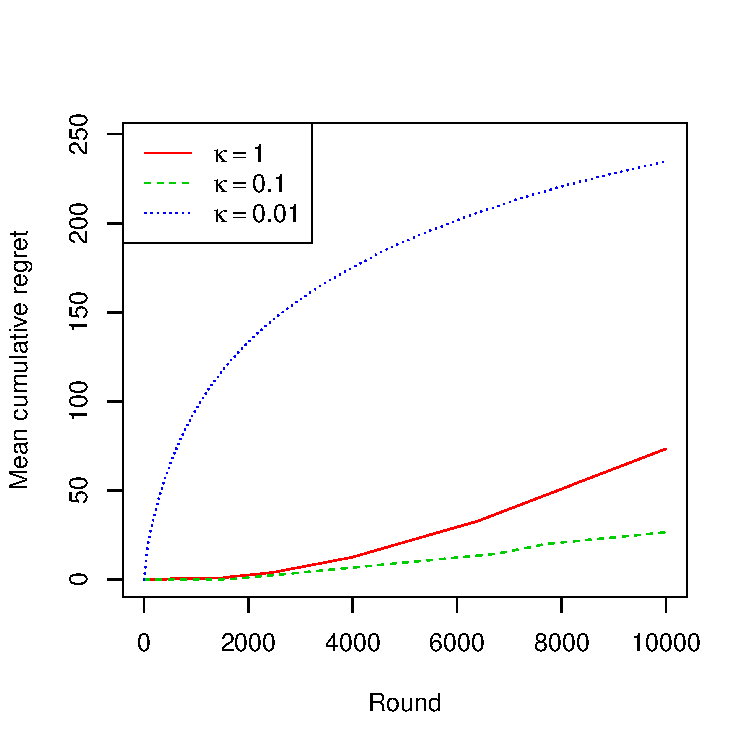
\includegraphics[width=\linewidth]{FigNHANES_bene.pdf}
\caption{Mean cumulative regret of MND-B UCB in the semi-synthetic NHANES experiment over 100 runs (red solid: $\kappa=1$; green dashed: $\kappa=0.1$; blue dotted: $\kappa=0.01$).}\label{fig:nhanesB}
\end{minipage}\hfill
\begin{minipage}[t]{.48\textwidth}\centering
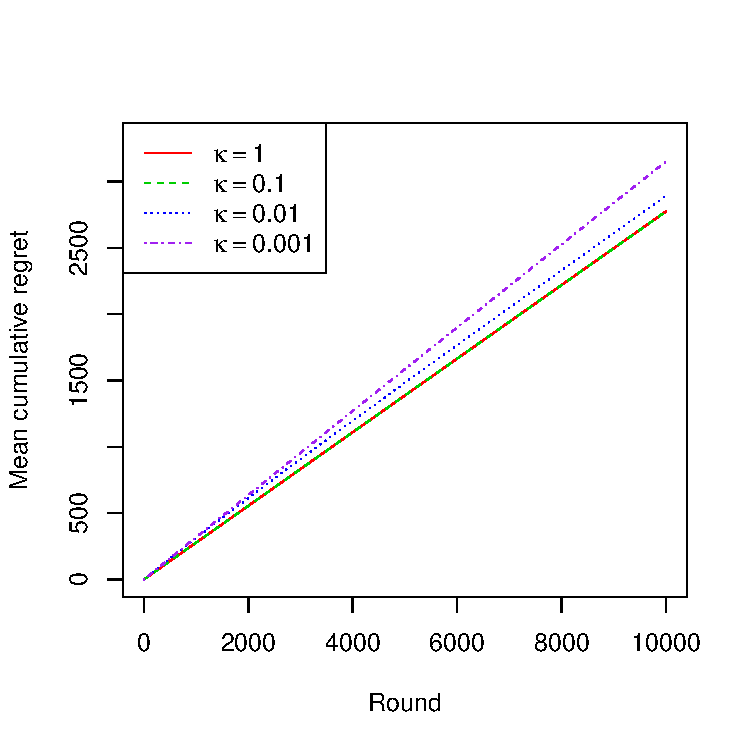
\includegraphics[width=\linewidth]{FigNHANES_harm.pdf}
\caption{Mean cumulative regret of MND-H UCB in the semi-synthetic NHANES experiment over 100 runs (red solid: $\kappa=1$; green dashed: $\kappa=0.1$; blue dotted: $\kappa=0.01$).}\label{fig:nhanesH}
\end{minipage}
\end{figure}

\begin{table}[tb]
\centering
\caption{Real cohort used in the semi-synthetic experiment: insulin-naive adults with diagnosed diabetes and HbA1c $\ge 7\%$ in NHANES 2017--2018 ($n=229$). Median [interquartile range].}
\label{tab:nhanes_cohort}
\small
\begin{tabular}{lc}
\hline
Age (years) & 62.0 [53.0, 69.0] \\
Body weight (kg) & 86.2 [73.3, 102.4] \\
Baseline HbA1c (\%) & 7.8 [7.3, 8.9] \\
\hline
\end{tabular}
\end{table}

\begin{table}[tb]
\centering
\caption{Ground truth of each basal insulin dose in the semi-synthetic experiment, computed from $2\times10^6$ patients resampled from the NHANES cohort. Over-treated: the patient would also have reached the target at the next lower dose. Bold: the optimum of each criterion.}
\label{tab:nhanes_truth}
\small
\begin{tabular}{lccccc}
\hline
Dose (U/day) & 0 & 10 & 20 & 30 & 40 \\
\hline
$\theta^{\text{B}}$ (HbA1c $\le7\%$) & 0.055 & 0.566 & 0.709 & 0.779 & \textbf{0.823} \\
$\theta^{\text{H}}$ ($6\%<$ HbA1c $\le7\%$) & 0.055 & 0.556 & \textbf{0.638} & 0.632 & 0.609 \\
$\theta^{\text{MNB}}$ & 0.231 & \textbf{0.511} & 0.143 & 0.070 & 0.044 \\
$\theta^{\text{MNH}}$ & 0.233 & \textbf{0.510} & 0.143 & 0.070 & 0.044 \\
HbA1c $\le6\%$ & 0.000 & 0.010 & 0.071 & 0.147 & 0.215 \\
Over-treated & 0.000 & 0.055 & 0.566 & 0.709 & 0.779 \\
\hline
\end{tabular}
\end{table}

\begin{table}[tb]
\centering
\caption{Most frequently chosen dose in the semi-synthetic experiment ($T=10000$, $T^{\text{initial}}=100$, 100 runs) and the proportion of runs in which it is chosen. The MND-B is 10 U/day and the MND-H is 10 U/day.}
\label{tab:nhanes_choice}
\small
\resizebox{\textwidth}{!}{%
\begin{tabular}{lc|lc}
\hline
Algorithm (Benefit) & Chosen dose & Algorithm (Harmless) & Chosen dose \\
\hline
MND-B UCB ($\kappa=1$) & \textbf{10 U/day} (97\%) & MND-H UCB ($\kappa=1$) & 0 U/day (100\%) \\
MND-B UCB ($\kappa=0.1$) & \textbf{10 U/day} (99\%) & MND-H UCB ($\kappa=0.1$) & 0 U/day (100\%) \\
MND-B UCB ($\kappa=0.01$) & \textbf{10 U/day} (100\%) & MND-H UCB ($\kappa=0.01$) & 0 U/day (100\%) \\
\hline
MND-B UCB without confirmation task & \textbf{10 U/day} (98\%) & MND-H UCB without confirmation task & 0 U/day (100\%) \\
Benefit UCB & 40 U/day (100\%) & Harmless UCB & 20 U/day (78\%) \\
MED-TS for benefit ($\phi=0.5$) & \textbf{10 U/day} (100\%) & MED-TS for harmless ($\phi=0.5$) & \textbf{10 U/day} (100\%) \\
MED-TS for benefit ($\phi=0.7$) & 20 U/day (81\%) & MED-TS for harmless ($\phi=0.7$) & 20 U/day (70\%) \\
MED-TS for benefit ($\phi=0.8$) & 40 U/day (100\%) & MED-TS for harmless ($\phi=0.8$) & 20 U/day (69\%) \\
TS\_A for benefit ($\phi=0.5$) & \textbf{10 U/day} (100\%) & TS\_A for harmless ($\phi=0.5$) & \textbf{10 U/day} (100\%) \\
TS\_A for benefit ($\phi=0.7$) & 20 U/day (100\%) & TS\_A for harmless ($\phi=0.7$) & 20 U/day (64\%) \\
TS\_A for benefit ($\phi=0.8$) & 30 U/day (61\%) & TS\_A for harmless ($\phi=0.8$) & 20 U/day (63\%) \\
\hline
\end{tabular}}
\end{table}

\begin{table}[tb]
\centering
\caption{In-trial outcomes over the $T=10000$ trial patients, averaged over 100 runs: mean basal insulin dose, and the proportions of patients who reached the target (HbA1c $\le7\%$), were driven to over-intensive control (HbA1c $\le6\%$), and were over-treated (would also have reached the target at the next lower dose).}
\label{tab:nhanes_clinical}
\small
\begin{tabular}{lcccc}
\hline
Algorithm & Mean dose (U/day) & HbA1c $\le7\%$ & HbA1c $\le6\%$ & Over-treated \\
\hline
MND-B UCB ($\kappa=0.01$) & 9.4 & 53.0\% & 1.0\% & 5.5\% \\
MND-H UCB ($\kappa=0.01$) & 7.3 & 24.8\% & 3.2\% & 15.4\% \\
MND-H UCB ($\kappa=0.003$) & 17.8 & 52.8\% & 7.9\% & 37.6\% \\
MND-H UCB ($\kappa=0.001$) & 23.1 & 66.9\% & 10.3\% & 48.7\% \\
Benefit UCB & 36.7 & 80.7\% & 19.2\% & 74.7\% \\
Harmless UCB & 26.3 & 74.4\% & 11.9\% & 61.6\% \\
MED-TS for benefit ($\phi=0.7$) & 23.1 & 73.0\% & 9.5\% & 60.7\% \\
TS\_A for benefit ($\phi=0.7$) & 20.4 & 71.1\% & 7.5\% & 56.6\% \\
\hline
\end{tabular}
\end{table}

